\documentclass{article}
\usepackage{amsmath}
\usepackage{graphicx}
\author{Chang Liu ~\\ chang\_liu@student.uml.edu}
\title{91.673 Advanced Database Systems Homework4}
\begin{document}

\maketitle

\section{Problem 1:Exercise 5.1.2}

\textbf{Exercise 5.1.2}: Compute the PageRank of each page in Fig. 5.7, assuming $\beta$ = 0.8. ~\\
\begin{center}
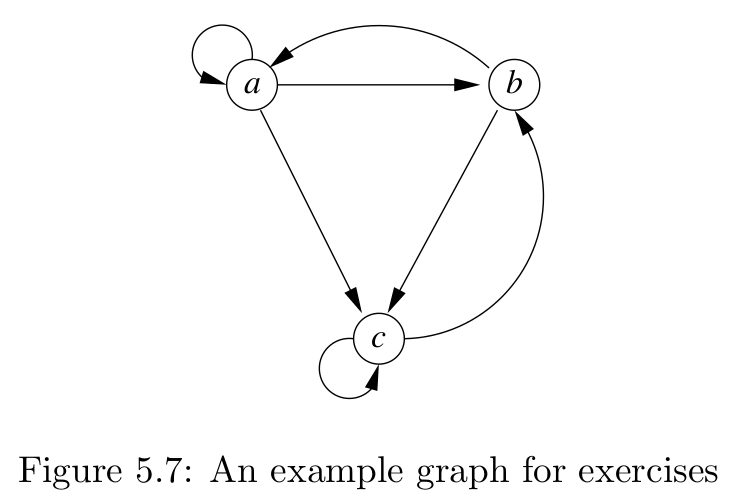
\includegraphics[scale=0.3]{hw3-figure5_7.png}
\end{center}

\textbf{Answer:}

According to the PageRank equation: $$r_j = \sum\limits_{i \rightarrow j}{\beta\frac{r_i}{d_i} + (1-\beta)\frac{1}{N}}$$

First, try to build the stochastic adjacency matrix $M$ using the following relationship about their importance $r_i$
$$r_a = r_b/2 + r_a/3$$
$$r_b = r_a/3 + r_c/2$$
$$r_c = r_a/3 + r_b/2 + r_c/2$$

The we can get:
\begin{equation}
M = \begin{pmatrix} 1/3 & 1/2 & 0 \\ 1/3 & 0 & 1/2 \\ 1/3 & 1/2 & 1/2 \end{pmatrix} 
\end{equation}

Add their result and get the final matrix as follows:

$$r_j = \sum\limits_{i \rightarrow j}{\begin{pmatrix} 1/3 & 7/15 & 1/15 \\ 1/3 & 1/15 & 7/15 \\ 1/3 & 7/15 & 7/15 \end{pmatrix}}$$

Using the equation $r = M * r$, do the iteration multiple times, and then we can get the following result: ~\\
1st iteration: r = (0.33 0.2 0.467) \\
2nd iteration: r = (0.26 0.2 0.52) \\
3rd iteration: r = (0.29 0.18 0.56) \\
... \\
100th iteration: r = (0.2121 0.1515 0.6364) \\

After that it's quite stable, so the PageRank of a is \textbf{0.21}, b is \textbf{0.15}, c is \textbf{0.64} 



\section{Problem 2: Exercise 5.3.1}
\textbf{Exercise 5.3.1}: Compute the topic-sensitive PageRank for the graph of Fig.5.15, assuming the teleport set is:

(a) A only.

(b) A and C.


\begin{center}
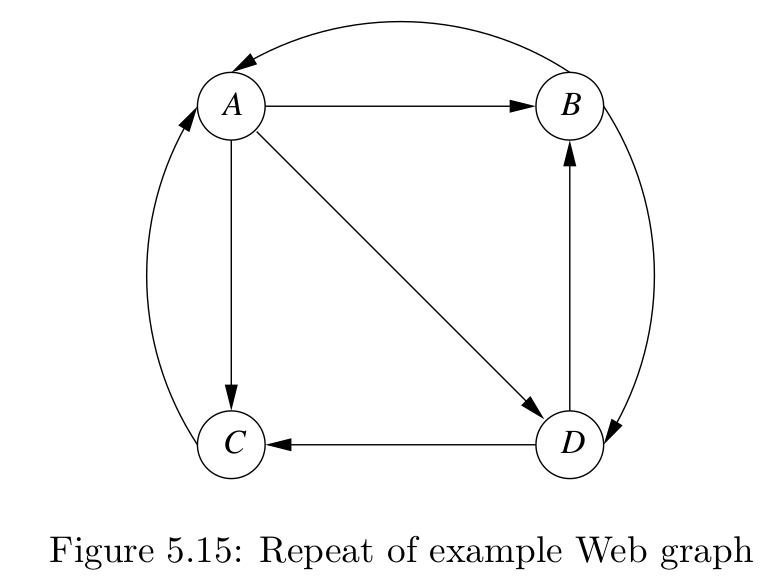
\includegraphics[scale=0.3]{hw4_figure_5_15.png}
\end{center}


\textbf{Answer:}

Here for the topic-sensitive, we should consider the topic when using the random jump, which means that only jumping to the node that related with the topic, the general form is $$v' = \beta{}Mv+(1-\beta)e_s/|S|$$

As the first problem shows, first try to build the matrix M, which is:
$$M = \begin{pmatrix} 0 & 1/2 & 1 & 0 \\ 1/3 & 0 & 0 & 1/2 \\ 1/3 & 0 & 0 & 1/2 \\ 1/3 & 1/2 & 0 & 0\end{pmatrix}$$

(a) For A only, the vector should be (1 0 0 0), as A is the only case, use the equation above with $\beta{}=0.8$, try to start as the vector $v=\begin{matrix} 1 & 0 & 0 & 0\end{matrix}$, since A relates to the topic. NOTE that the initial distribution has no effect on the limit or the final result, doing multiple iterations and the final value reaches:


\begin{center}
v = (0.4286 0.1905 0.1905 0.1905)
\end{center}

so the topic-sensitive PageRank for a, b, c, d is \textbf{0.43}, \textbf{0.19}, \textbf{0.19}, \textbf{0.19} respectively.
~\\

(b) For A and C, the biased vector should be (1/2 0 1/2 0), other functions are the same, using the same method we can get:

\begin{center}
v = (0.3857  0.1714  0.2714 0.1714)
\end{center}

so the topic-sensitive PageRank for a, b, c, d is \textbf{0.39}, \textbf{0.17}, \textbf{0.27}, \textbf{0.17} respectively.

For some details, please refer to my code.


\section{Problem 3: Exercise 6.1.5}

\textbf{Exercise 6.1.5}: For the data of Exercise 6.1.1, what is the confidence of the
following association rules?

(a) $\{5, 7\} \rightarrow  2$.

(b) $\{2, 3, 4\} \rightarrow 5$.

~\\
\textbf{Answer:}

According to the definition of confidence, $$conf(I \rightarrow j) = \frac{support(I \bigcup j)}{support(I)}$$

calculate the probability of the two sets and then we can get the confidence.
~\\

(a) For this case, the probability of showing item 5 and 7 in the same basket is that the basket number can be divided by 5 AND 7, so it can only be 35 and 70 in these two cases. $p(support(I)) = 2/100$.

And the probability of showing item 2, 5, 7 in the same time can only be the case that basket number is 70, the so probability is $p(support(I \bigcup j)) = 1/100$.

According to the above equation, the confidence should be 0.5 after their division.

~\\
(b) Using the same method, in the set I, the basket can be $\{$12, 24, 36, 48, 60, 72, 84, 96$\}$, so probability is $p(support(I)) = 8/100$. And the probability of I with j is $p(support(I \bigcup j)) =  1/100$, as the basket can only be 60, so the confidence in this case should be 1/8 = 0.125.



\section{Problem 4: Exercise 6.2.6 (a)}

\textbf{Exercise 6.2.6}: Apply the A-Priori Algorithm with support threshold 5 to the data of:

(a) Exercise 6.1.1.



\section{Problem 5: Exercise 7.3.1}


\textbf{Exercise 7.3.1}: For the points of Fig. 7.8, if we select three starting points using the method
of Section 7.3.2, and the first point we choose is (3,4), which other points are selected.




\end{document}

